% ID: SEL-D0012-BB-E03
% ESTADO: validada. S013; tres pasadas del mismo autor, sin segundo revisor.
\textbf{a) Continuidad.}\par\nopagebreak[4]
Ambas ramas son polinómicas. Sólo hay que revisar la unión $x=1$:
\[
a+b=1-b+a\quad\Longleftrightarrow\quad\boxed{b=\frac12.}
\]
Esta condición sirve para cualquier $a$ y hace coincidir los límites laterales y $f(1)$.

\textbf{b) Derivabilidad con b=1/2.}\par\nopagebreak[4]
La continuidad ya está garantizada. Las derivadas laterales son $a$ y $2-b=3/2$, luego
\[
\boxed{a=\frac32.}
\]
Así queda derivable en todo $\mathbb R$.

\textbf{c) Monotonía y extremos cuando a<0.}\par\nopagebreak[4]
Para $x<1$, $f'=a<0$. Para $x>1$, $f'=2x-1/2>0$. Como es continua en la unión, \textbf{decrece en $(-\infty,1]$ y crece en $[1,+\infty)$}. Hay un único mínimo relativo y absoluto, en
\[
\boxed{x=1,\qquad f(1)=a+\frac12.}
\]
No hay máximos: ambas colas tienden a $+\infty$. En $1$ no es derivable para $a<0$, pero eso no impide el mínimo. El cero $x=1/4$ de la derivada de la expresión cuadrática queda fuera de su tramo y no es punto crítico de esta función.

\textbf{d) Región y área para a=0.}\par\nopagebreak[4]
En $[0,1)$, $f=1/2$; en $[1,2]$, $f=x^2-x/2\geq1/2$. Toda la región queda sobre el eje, por lo que no hay que cambiar signos.
\begin{center}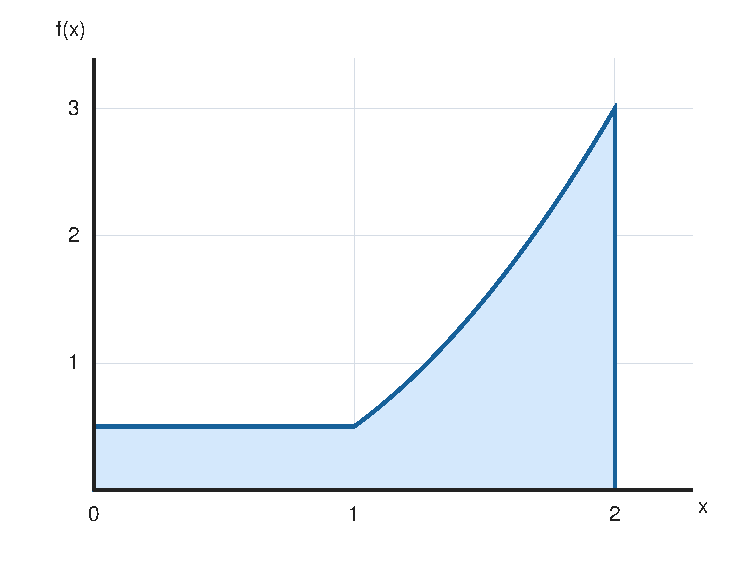
\includegraphics[width=0.56\linewidth]{recursos/figuras/s013-area.pdf}\end{center}
\[
\begin{aligned}
\mathcal A&=\int_0^1\frac12\,dx+\int_1^2\left(x^2-\frac x2\right)\,dx\\
&=\frac12+\left[\frac{x^3}{3}-\frac{x^2}{4}\right]_1^2
=\frac12+\frac{19}{12}=\boxed{\frac{25}{12}\text{ unidades cuadradas}.}
\end{aligned}
\]
Se ha dividido la integral en el cambio de fórmula, aunque la función sea continua allí.
